\documentclass{standalone}
\usepackage{tikz}
\usepackage{ctex,siunitx}
\usepackage{tkz-euclide}
\usepackage{amsmath}
\usetikzlibrary{patterns, calc}
\usetikzlibrary {decorations.pathmorphing, decorations.pathreplacing, decorations.shapes,}
\begin{document}
\small
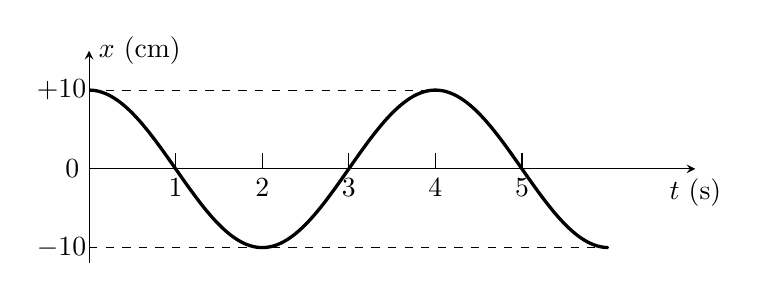
\begin{tikzpicture}[>=stealth, xscale=0.7, domain=0:3*pi, samples=200]
  \draw [->](0,0)node [left]{$0$}--(11,0) node [below]{$t$ (\unit{s})};
  \draw [->](0,-1.2)--(0,1.5) node [right]{$x$ (\unit{cm})};
  \draw [very thick]  plot (\x,{cos(\x r)});
  \draw [dashed](0, 1) -- (2*pi, 1);  
  \draw [dashed](0,-1) -- (3*pi, -1);     
  \foreach \x in{1,2,...,5}
  {
  \draw(\x*pi/2, 0)node [below]{\x}--(\x*pi/2, 0.2);
  }
  \node at (-.5,1){$+10$};\node at (-.5,-1){$-10$};
\end{tikzpicture}
\end{document}